
\documentclass[10pt]{beamer} 
\usetheme[pageofpages=of,% String used between the current page and the
          % total page count.
          alternativetitlepage=true,% Use the fancy title page.
          %titlepagelogo=coca,% Logo for the first page.
          titleline=true
          ]{Torino}
%\usetheme{Frankfurt}
\usecolortheme{chameleon}

\usepackage{graphicx,hyperref,url}
\usepackage[utf8]{inputenc}
\usepackage[T1]{fontenc}
\usepackage[portuges,brazilian]{babel}
%%%\usepackage{wrapfig}
\usepackage{caption}
\usepackage{subfigure}
%\usepackage{subcaption}
\usepackage{latexsym}
\usepackage{amssymb, amsmath}
\usepackage{multicol}
\usepackage{pifont}%,bbding}%%,dingbat} %%% ver manual de simbolos
\usepackage[final]{listings}
\usepackage{comment}


\definecolor{azulclaro}{rgb}{0.9,0.9,0.9}
\definecolor{mygreen}{rgb}{0,0.6,0}
\definecolor{mygray}{rgb}{0.5,0.5,0.5}
\definecolor{mymauve}{rgb}{0.58,0,0.82}
\definecolor{darkgray}{rgb}{.4,.4,.4}
\definecolor{purple}{rgb}{0.65, 0.12, 0.82}

\newcommand{\minizinc}{MiniZinc}

\lstset{ 
  %  label={pgm_ex01},
    backgroundcolor=\color{azulclaro}, 
    language=erlang, %%Miranda,%%Perl,%%%Python, %%Mercury,
    showstringspaces=false,
    basicstyle=\bf\scriptsize\ttfamily,
%%      basicstyle= \footnotesize %%% TESTAR
%%      keywordstyle=\bfseries\color{green!40!black},
    keywordstyle=\textbf{\color{mygreen}}, 
    otherkeywords={*, \%, array, constraint, solve, output,  show, "/\", satisfy, set, of, if, then, elseif, float, search},
%%  keywordstyle=\color{blue},       % keyword style
%%    commentstyle=\itshape\color{purple!40!black},
      commentstyle=\color{orange},    % comment style
      identifierstyle=\color{blue},
      stringstyle=\color{orange},
      stringstyle=\color{mymauve},
      numbers=left,  % where to put the line-numbers; possible values are (none, left, right)
      numbersep=5pt,   % how far the line-numbers are from the code
      numberstyle=\tiny\color{magenta},
      keepspaces=true      
    % %caption={LEGENDA no source PASCAL ficou OK},
}


\graphicspath{{/home/ccs/Dropbox/figs_genericas/}{figuras/}{/home/ccs/Dropbox/CCS/picat}}
\DeclareGraphicsExtensions{.pdf,.png,.jpg}
%Global Background must be put in preamble
%\usebackgroundtemplate{\includegraphics[width=\paperwidth]{amarelinho.pdf}}
%%% \begin{frame}[allowframebreaks=0.8]

% The log drawn in the upper right corner.

%\logo{\centering
%\includegraphics[height=0.050\paperheight]{figuras/logo_SBPO_Peixe.png}
%%\hspace{9.6cm}
%\includegraphics[height=0.027\paperheight]{figuras/logo_udesc_horizontal.jpg}


%%%%%%%%%%%%%%%%%%%%%%%%%%%%%%%%%%%%%%%%%%%%%%%%%%%%%%%%%%%%%%%%%%%%%


\title[Picat]{\fontsize{20}{30}\selectfont \textcolor{black}{Sistemas Multiagentes}}

\author[]{Claudio Cesar de Sá\\
     {\small \url{claudio.sa@udesc.br}}}

\institute[UDESC]{
    Departamento de Ci\^encia da Computa\c{c}\~ao \\
    Centro de Ci\^encias e Tecnol\'ogias\\
   Universidade do Estado de Santa Catarina}

%%%%%%%%%%%%%%%%%%%%%%%%%%%%%%%%%%%%%%%%%%%%%%%%%%%%%%%%%%%%%%%%%%%%%

\begin{document}

\begin{frame}
    \titlepage
\end{frame}

%%%%%%%%%%%%%%%%%%%%%%%%%%%%%%%%%%%%%%%%%%%%%%%%%%%%%%%%%%%%%%%%%%%%%

\begin{frame}[fragile]
\frametitle{Sumário}
\tableofcontents
\end{frame}


\section{Introdução}
\begin{frame}

    \frametitle{Histórico}

    \begin{itemize}
      \item 
      \item 
      \item 
    \end{itemize}
\end{frame}



\subsection{O Curso}
\begin{frame}

    \frametitle{Conteúdo do Curso}

    \begin{itemize}
      \item Conceitos de SMA (há muitos correlacionados há áreas diversas)
      \item Ferramentas: Netlogo e Picat
      \item Aplicação: voces escolhem
      \item Um artigo
      
    \end{itemize}
\end{frame}

\subsection{Ferramentas}
\begin{frame}

    \frametitle{Ferramentas}

    \begin{itemize}
      \item PICAT (com suporte)
      \item NETLOGO
       \url{http://ccl.northwestern.edu/netlogo/docs/} (escondido in WEB)
      
    \end{itemize}
\end{frame}


\subsection{Avaliação}
\begin{frame}

    \frametitle{Avaliação}

    \begin{itemize}
      \item Duas provas (conceituais) -- 25\%
      \item Exercícios de laboratório  -- 10\%
      \item Implementação de um protótipo  -- 20\%
      \item Apresentação de um artigo estudado sobre SMA -- 15\%
      \item O artigo (resultados da implementação)  -- 30\%
      \item Para o artigo: muito material será fornecido em \LaTeX ...
       
      
    \end{itemize}
\end{frame}



\subsection{Dinâmica}
\begin{frame}

    \frametitle{Dinâmica de Aula}

    \begin{itemize}
      \item Teoria na parte da manhã -- 10:00 hrs -- K-107
      \item \textit{Ralação} a tarde
      
    \end{itemize}
\end{frame}



\section{Introdução aos SMAs}

\begin{frame}

  \frametitle{Motivando aos SMAs}
    
    
\begin{figure}[!ht]
\centering
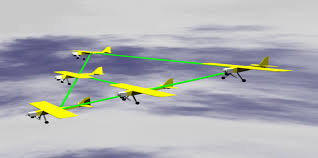
\includegraphics[height =.6\textheight,width=.7\textwidth]{figuras/agentes_vizinhos01.jpeg}
\caption{Observe o sentido das flechas --  e  o foco da missão}
%\label{ag_01}
\end{figure}
    
    
\end{frame}


\begin{frame}
\frametitle{Motivando aos SMAs}

\begin{figure}[!ht]
\centering
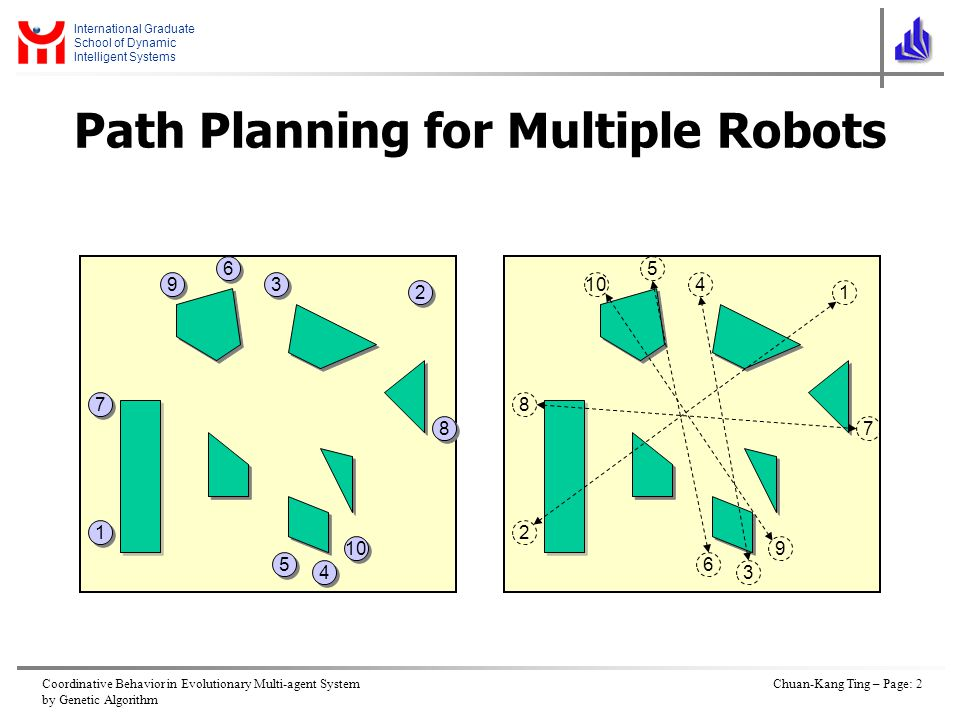
\includegraphics[height =.6\textheight,width=.7\textwidth]{figuras/agentes_vizinhos02.jpeg}
%\caption{Arquitetura clássica}
%\label{ag_01}
\end{figure}
\end{frame}
%%%%%%%%%%%%%%%%%%%%%%%%%%%%%%%%%%%%%%%%%%%%%%%%%%%%%%%%%%%%%%%%%

\begin{frame}

  \frametitle{Motivando aos SMAs}

\begin{figure}[!ht]
\centering
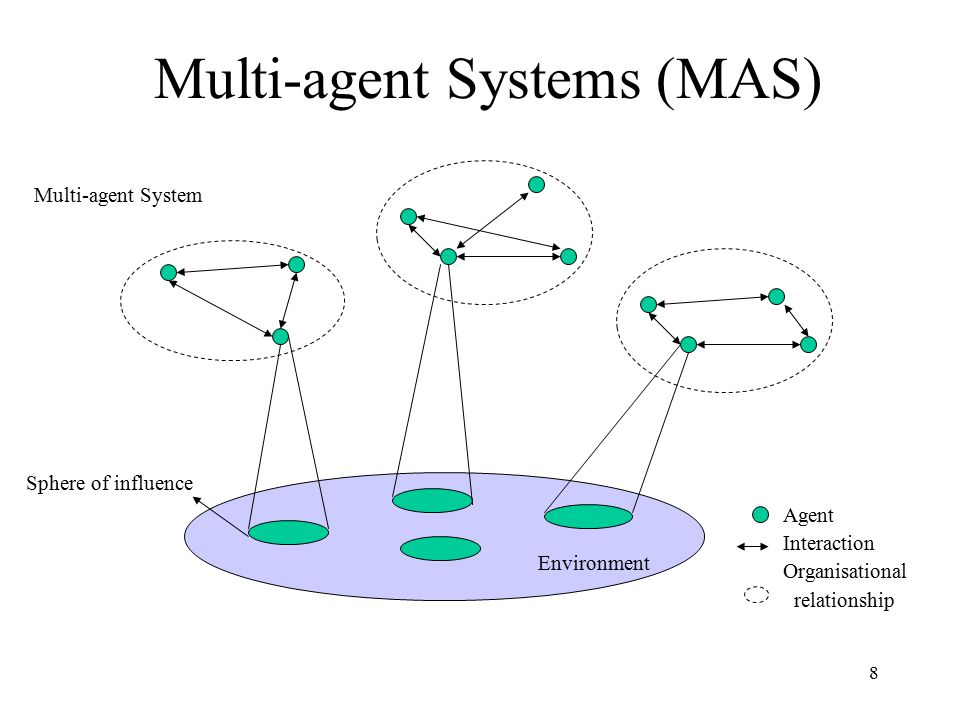
\includegraphics[height =.6\textheight,width=.7\textwidth]{figuras/agentes_vizinhos03.jpeg}
\caption{Arquitetura clássica -- comunidade de agentes $\equiv $   SMA}
%\label{ag_01}
\end{figure}
 
\end{frame}
%%%%%%%%%%%%%%%%%%%%%%%%%%%%%%%%%%%%%%%%%%%%%%%%%%%%%%%%%%%%%%%%%


\subsection{Motivação aos SMAs}
\begin{frame} [allowframebreaks=0.9]

    \frametitle{Motivação I}
    Projetar e construir sistemas multiagentes é uma tarefa difícil, pois:
    \begin{itemize}
    \pause
      \item Apresenta todos os problemas já conhecidos 
dos sistemas distribuídos e concorrentes.
\pause
      \item Dificuldades adicionais surgem da flexibilidade 
e complexidade das interações
    
    \end{itemize}
\end{frame}



\begin{frame}
\frametitle{Esta complexidade por um DFD por agente x ações:}
  
  \begin{figure}[!ht]
  \centering
  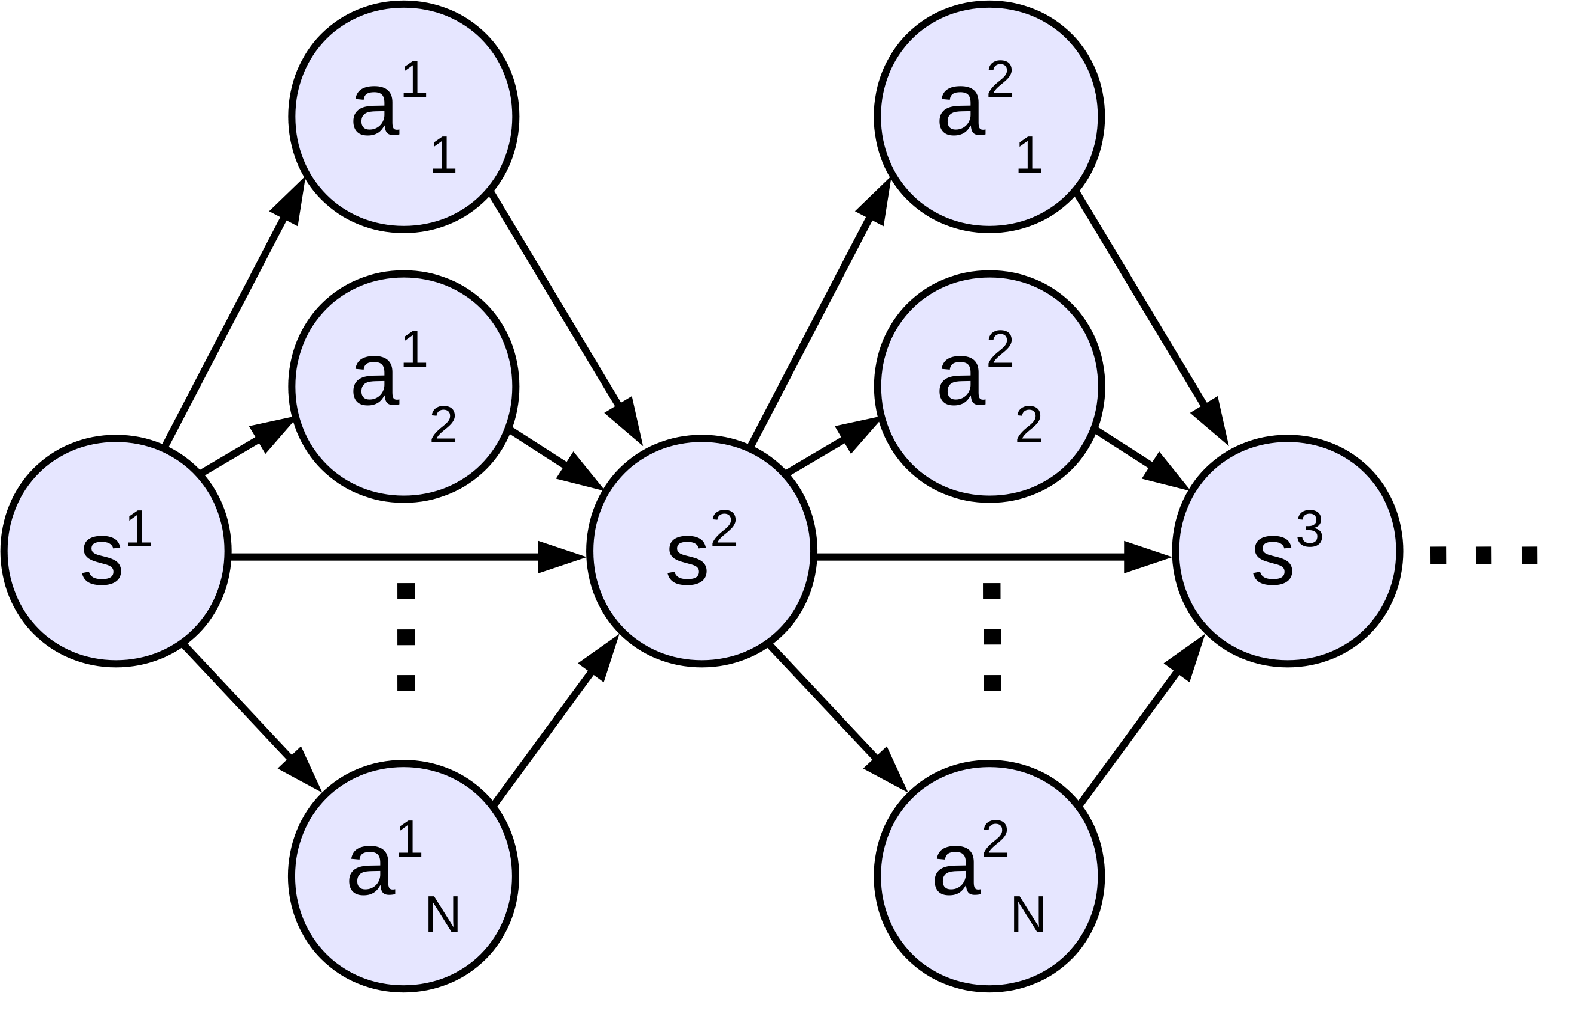
\includegraphics[height =.6\textheight,width=.7\textwidth]{figuras/mudando_estados01.png}
  \caption{Complexidade via DFD de um SMA (agentes) $\times $ ações $\equiv $ um único estado}
%\label{ag_01}
\end{figure}
   
\end{frame}




\begin{frame}

    \frametitle{Motivação II}
   Dois principais impedimentos técnicos, pois:
    \begin{itemize}
    \pause
      \item Inexistência de uma metodologia sistemática para 
      claramente especificar e estruturar aplicações SMA.
     \pause
      \item Inexistência de ferramentas e ambientes de 
desenvolvimento de SMA com qualidade industrial.
    
    \end{itemize}
\end{frame}

%%%%%%%%%%%%%%%%%%%%%%%%%%%%%%%%%%%%%%%%%%%%%%%%%%%%%%%%%%%%%%%%%%%%%%%%

\subsection{Os Elementos de SMAs}



\begin{frame}[allowframebreaks=0.9]

    \frametitle{Os Elementos de SMAs}
   
   \begin{description}
     \item[Projeto de Agente:] 
     
    \item[Ambiente:]
          
   \item[Percepção:]
               
 \item[Controle:]
                    
  \item[Conhecimento:]
                          
  \item[Comunicação:]
          
   \end{description}
   
   
\end{frame}




%%%%%%%%%%%%%%%%%%%%%%%%%%%%%%%%%%%%%%%%%%%%%%%%%%%%%%%%%%%%%%%%%%%%%%%%
\section{Agentes Racionais}
\begin{frame}

    \frametitle{Características aos SMAs}
    \begin{itemize}
    \pause
      \item 
\pause
      \item cap 2
    
    \end{itemize}
\end{frame}






\subsection{Agentes Racionais}

\begin{frame}

  \frametitle{Agente em seu ambiente}
    
\begin{figure}[!ht]
  \centering
  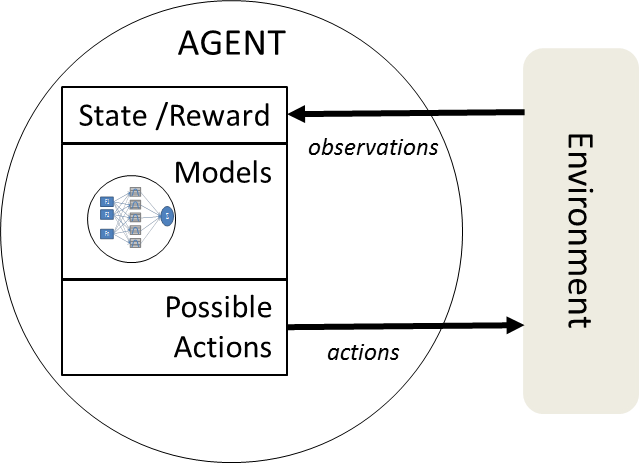
\includegraphics[height =.6\textheight,width=.7\textwidth]{figuras/agente_ambiente_ciclo.png}
  \caption{Ciclo do agente}
%\label{ag_01}
\end{figure}
    
\end{frame}



\begin{frame}

  \frametitle{Arquitetura clássica de um agente reflexivo}
    
\begin{figure}[!ht]
\centering
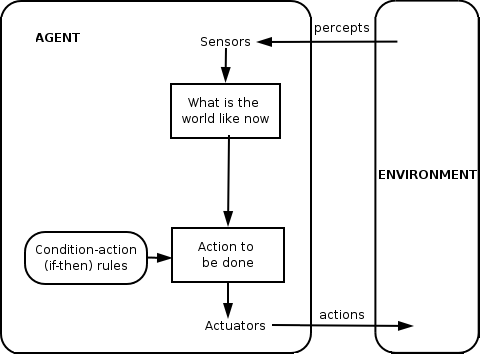
\includegraphics[width=.6\textwidth]{figuras/agent-reflexivo.png}
\caption{Arquitetura clássica}
\label{ag_01}
\end{figure}
    
\end{frame}


\begin{frame}

  \frametitle{Arquitetura clássica de um agente que \textit{aprende} -- desejável}
    
\begin{figure}[!ht]
\centering
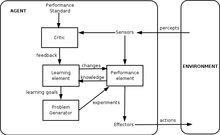
\includegraphics[width=.6\textwidth]{figuras/agent-learning.png}
\caption{Arquitetura clássica}
\label{ag_01}
\end{figure}
    
\end{frame}


\section{Estratégias de Jogos}
\begin{frame}

    \frametitle{Teoria de Jogos}
    \begin{itemize}
    \pause
      \item 
\pause
      \item cap 3
    
    \end{itemize}
\end{frame}


\section{Coordenação}
\begin{frame}

    \frametitle{Coordenação}
    \begin{itemize}
    \pause
      \item 
\pause
      \item cap 4
    
    \end{itemize}
\end{frame}

\subsection{Exemplos de Coordenação SMAs}

\begin{frame}
\frametitle{Exemplo de Coordenação SMAs}

\begin{figure}[!ht]
\centering
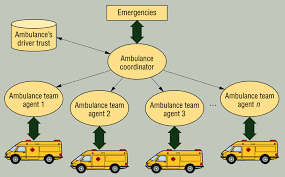
\includegraphics[height =.6\textheight,width=.7\textwidth]{figuras/coordenacao_agentes01.png}
\caption{Coordenação de agentes $\equiv $   SMA}
%\label{ag_01}
\end{figure}
 \end{frame}





\begin{frame}
\frametitle{Exemplo de Coordenação SMAs}

\begin{figure}[!ht]
\centering
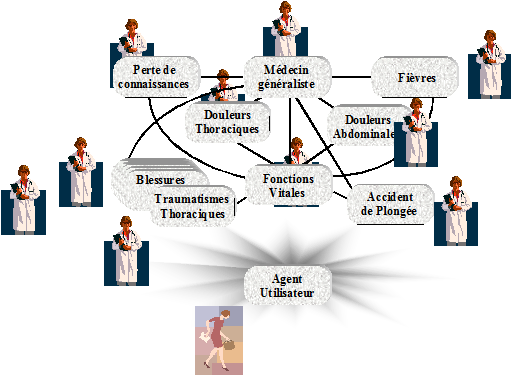
\includegraphics[height =.6\textheight,width=.7\textwidth]{figuras/coordenacao_agentes02.png}
\caption{Coordenação de agentes $\equiv $   SMA}
%\label{ag_01}
\end{figure}
 
\end{frame}

\section{Teoria de Jogos Aplicado a SMA}
\begin{frame}

    \frametitle{Teoria de Jogos Aplicado a SMA}
    \begin{itemize}
    \pause
      \item $\prod^{n}_{x=1} \neq  \prod_{x=1}^{n+1}$
      \item  \url{https://www.codecogs.com/latex/eqneditor.php}
      \item \url{http://www.hostmath.com/}
      

      \pause
      \item cap 6
    
    \end{itemize}
\end{frame}




\section{Projetos de SMAs}
\begin{frame}

    \frametitle{Mecanismos de Projetos}
    \begin{itemize}
    \pause
      \item 
\pause
      \item cap 6
    
    \end{itemize}
\end{frame}




\section{Implementação de SMAs}
\begin{frame}

    \frametitle{Implementação de Agentes}
    \begin{itemize}
    \pause
      \item 
\pause
      \item xxxxxxxxxxxx
    
    \end{itemize}
\end{frame}



\section{Aprendizagem}
\begin{frame}

    \frametitle{Aprendizagem}
    \begin{itemize}
    \pause
      \item 
\pause
      \item cap 7
    
    \end{itemize}
\end{frame}




%%%%%%%%%%%%%%%%%%%%%%%%%%%%%%%%%%%%%%%%%%%%%%%%%%%%%%%%%%%%%%%%%%%%%

\section{Conclusão}
\begin{frame}
    \frametitle{Conclusão}
    \begin{itemize}
    \item .
    \end{itemize}
\end{frame}

%%%%%%%%%%%%%%%%%%%%%%%%%%%%%%%%%%%%%%%%%%%%%%%%%%%%%%%%%%%%%%%%%%%%%

%\section{Referências}
\begin{frame}
    \frametitle{Referências}
    \begin{itemize}
     \item \url{https://github.com/claudiosa/CCS/tree/master/sma}
     \item \url{}
    \end{itemize}
\end{frame}

%%%%%%%%%%%%%%%%%%%%%%%%%%%%%%%%%%%%%%%%%%%%%%%%%%%%%%%%%%%%%%%%%%%%%

\end{document}
